% \documentclass[twoside]{EOSC350TBL2017} %         DON'T SHOW ANSWERS
\documentclass[twoside]{EOSC454} %      SHOW ANSWERS

\newcommand{\TODO}[1]{{\color{red} #1}}

% LJH Comments: Why 31.6 mS / m ?


% === LAB INFO =================== %
%\title{Team TBL \# 4: Detecting lost squardon \\ from Sensors \& Software}
\title{EOSC 454 / 556B Assignment 2: Linear Inverse Problem}
\dueDate{February 29, 2024}

\setlength{\parskip}{10pt}
\setlength\parindent{0pt}

% ====================================== %
% ======== DOCUMENT ==================== %
% ====================================== %

\begin{document}
\figdir{./Figures} % Figure directory

% ======== OVERVIEW AND INTRO MATERIAL ===== %
\begin{framed}

% ---------------- OVERVIEW ---------------- %
\section*{Overview}

In this assignment, you will work with the linear problem that has kernels which are decaying exponential functions.

You are welcome to use the notebook that we wrote together in class as a starting point, but please be mindful that you should rename variables to be more descriptive and that the setup you will be asked to use will be different from the exercise that we completed in class.

Also, I highly recommend that you update the functions that we wrote so that each function only uses local variables and that there are no global variables.


% --------------- INSTRUCTIONS ------------- %


\section*{Instructions}
\sloppy

Please submit your assignment on canvas. In your submission, please include:
\begin{itemize}
    \item A write-up: this can be completed in word, LaTeX, Jupyter or similar. Please submit a PDF. For graduate students, I recommend that you work with LaTeX to build familiarity with it. For figure, please include axes labels, a legend (where appropriate), and a figure caption.

    \item Jupyter notebook / code: please submit a pdf of the notebook you wrote along with either (a) a zip file including the notebook and any additional python files you wrote, or (b) a link to a GitHub repository with your code
\end{itemize}

You are welcome to work with your classmates (and encouraged to do so!). You each must hand in your own work. Please indicate who you collaborated with in your report.


\end{framed}

\pagebreak

\question{
    In this question, we will set up the forward simulation using kernels that are decaying exponential functions.
    The kernel functions take the form
        \begin{equation}
        g_j(x) = e^{j p x} \cos(2 \pi j q x)
        \label{eq:kernels}
        \end{equation}
    and each datum is
        \begin{equation}
        d_j = \int_{v} g_j(x) m(x) dx
        \label{eq:datum}
        \end{equation}
    As we discussed in class, this can be written in discrete form as
        \begin{equation}
        \mathbf{d} = \mathbf{G}\mathbf{m}
        \label{eq:linear-problem}
        \end{equation}
}

\part{
    Create a function that generates the kernel functions $g(x)$ given scalar values for $j, p, q$ and a vector of locations $x$. Define a mesh with 100 cells with the domain $0 \leq x \leq 1$. Describe the roles of $p, q$ and $j$ in the nature of the kernel function (plots will be helpful)
}

\part{
    Design a model that consists of a Gaussian and a boxcar and use different parameters than we used in class (e.g. change the location of the boxcar / Gaussian, change the amplitude, make one have a negative amplitude, etc). Plot your model.
}

\part{
    Next create a function that builds the forward simulation matrix $\mathbf{G}$ and simulate data using 20 kernels with $p = -0.05$, $q = 0.1$, $0 \leq j \leq 30$, with the values for $j$ being evenly spaced. Create a plot with 3 subplots that show the model, kernels and data.
}

\part{
    In this part, we will examine the concept of sensitivity: how a change in the model impacts the data. For these examples, we can quantify the sensitivity using
    \begin{equation}
        \frac{\| \mathbf{d}(m_1) = \mathbf{d}(m_2) \|}{||\Delta m||}
        \label{eq:sensitivity}
    \end{equation}
    Where $m_1$ is your original model, $m_2$ is the new model, and $\Delta m$ is the change in the amplitude (of either the boxcar or Gaussian, independently).
    Change the amplitude of the boxcar, compute the sensitivity using equation \ref{eq:sensitivity}, plot the data, and comment on how a chance in the amplitude of the boxcar changes the data. Next repeat these steps changing the amplitude of the Gaussian.
}

\part{
    Now, we will look at how the kernels impact the sensitivity to features in the model. Make the kernel functions less oscillatory by decreasing $q$; use $q = 0.05$. Now change the amplitude of the boxcar and Gaussian independently. Describe how this impacts the data and quantify the sensitivity using equation \ref{eq:sensitivity}. What happens if the kernels are more oscillatory ($q = 0.2$)?
}

\part{
    Set $q=0.1$ again. Finally, create some examples that show how $p$ impacts sensitivity. Change $p$ to make the kernels decay more rapidly, and then less rapidly and describe how the data changes with changes in the model parameters in each scenario.
}

\question{
    In this question, we will set up the inverse problem. We will be solving a problem of the form
    \begin{equation}
        \min_{\mathbf{m}} \phi(\mathbf{m}) = \phi_d(\mathbf{m}) + \beta \phi_m (\mathbf{m})
    \label{eq:inverse-problem}
    \end{equation}
    where $\phi_d$ is the data misfit, given by
    \begin{equation}
      \phi_d(\mathbf{m}) = \| \mathbf{W}_d(\mathbf{G}\mathbf{m} - \mathbf{d}^{obs})\|^2
        \label{eq:inverse-problem}
    \end{equation}
    with $\mathbf{W}_d = \text{diag}(1/\mathbf{\epsilon})$ where $\mathbf{\epsilon} = [\epsilon_1, \epsilon_2, ... \epsilon_N]^\top$ is a vector containing the standard deviations of each datum.
    The model norm we will use consists of two parts, a ``smallness'' term and a first-order ``smoothness'' term. The continuous version is written as
    \begin{equation}
        \phi_m(m) = \alpha_s \int_x (m - m_{ref})^2 dx + \alpha_x \int_x \left(\frac{dm}{dx}\right)^2 dx
    \label{eq:model-norm-continuous}
    \end{equation}
    and the discrete version can be written as
    \begin{equation}
        \phi_m(\mathbf{m}) = \alpha_s \| \mathbf{W}_s (\mathbf{m} - \mathbf{m}_{ref})\|^2 + \alpha_x \| \mathbf{W}_x (\mathbf{m})\|^2
    \label{eq:model-norm-continuous}
    \end{equation}
}

\part{
    We will start by setting up all of the pieces that we need, beginning with the $\mathbf{W}_d$, $\mathbf{W}_s$ and $\mathbf{W}_x$ matrices. We programmed everything for $\mathbf{W}_d$ and $\mathbf{W}_s$ in class, and we talked about what the structure of $\mathbf{W}_x$ should look like. Write a small function to generate $\mathbf{W}_d$ given values for the standard deviations of the data. Write functions to generate $\mathbf{W}_s$ and $\mathbf{W}_x$ given the locations of the nodes of the mesh (e.g. the \texttt{x\_nodes} vector we created in class). Test the creation of the  matrices with a very small mesh (e.g. 4 cells) and very small number of data (e.g. 2 data points). Describe the shapes of each matrix and print the entries that they contain.
}

\part{
    Next, we will derive the system of equations that need to be solved to solve the inverse problem and recover a model $(\mathbf{\tilde{m}})$. For simplicity, you can assume $\mathbf{m}_{ref} = \mathbf{0}$ (as a bonus, keep $\mathbf{m}_{ref}$ in your derivation). We know that for a convex function, the minimum occurs when $\nabla \phi = 0$. Take the derivative of the objective function in equation \ref{eq:inverse-problem} and set that equal to 0. Derive the linear equations that need to be solved to estimate $\mathbf{m}.$
}

\part{
    Now, we will program a function to estimate a model given a observed data, estimates of the uncertainties on those data, and the parameters $\beta, \alpha_s, \alpha_x$. It is also a good idea to have this function take the matrix $\mathbf{G}$ so that it is easy to later play with the kernels. Create this function. Now we will use it to recover a model. Use the parameters for the kernels described in Q1c and add Gaussian random noise with a standard deviation of $10^{-2}$. Try two different scenarios:
    \begin{itemize}
        \item assign the correct standard deviations to the observed data and use $\alpha_s = 1$ and $\alpha_x = 0$. Choose a $\beta$-value that gives you $\phi_d\sim N$ where $N$ is the number of data.
        \item assign the correct standard deviations to the observed data and use $\beta=10^{3}$, $\alpha_s = 0$ and $\alpha_x = 1$. Choose a $\beta$-value that gives you $\phi_d\sim N$ where $N$ is the number of data.
    \end{itemize}
    Generate a plot with three panels that shows: (a) the true and recovered models, (b) the kernels, and (c) the observed and predicted data for each of these scenarios (it will be useful if you create a function for generating these plots that takes the true and recovered models, and $\mathbf{G}$ matrix). Specify the choice of $\beta$ and the resultant $\phi_d$-value (here, I am only looking for something that is the right order of magnitude, e.g. try $\beta=10^{2}, 10^3, 10^4, ...$. We will get more specific in the next questions.)
}



\question{
    In this question, we will plot and explore the Tikhonov curves. You will generate a plot that has 6 panels. One row should show the Tikhonov curves: $\phi_d$ vs. $\beta$, $\phi_m$ vs. $\beta$, and $\phi_d$ v.s. $\phi_m$ (be sure to plot $\beta$ as decreasing to the right, just as we did in class), and another row should show the true and recovered model, the kernels, and the predicted and observed data. It should look something like Figure \ref{fig:Tikhonov-curves-example} (note that your model might be different than mine, so the curves, model and data will all look different.)
    \begin{figure}[H]
        \begin{center}
        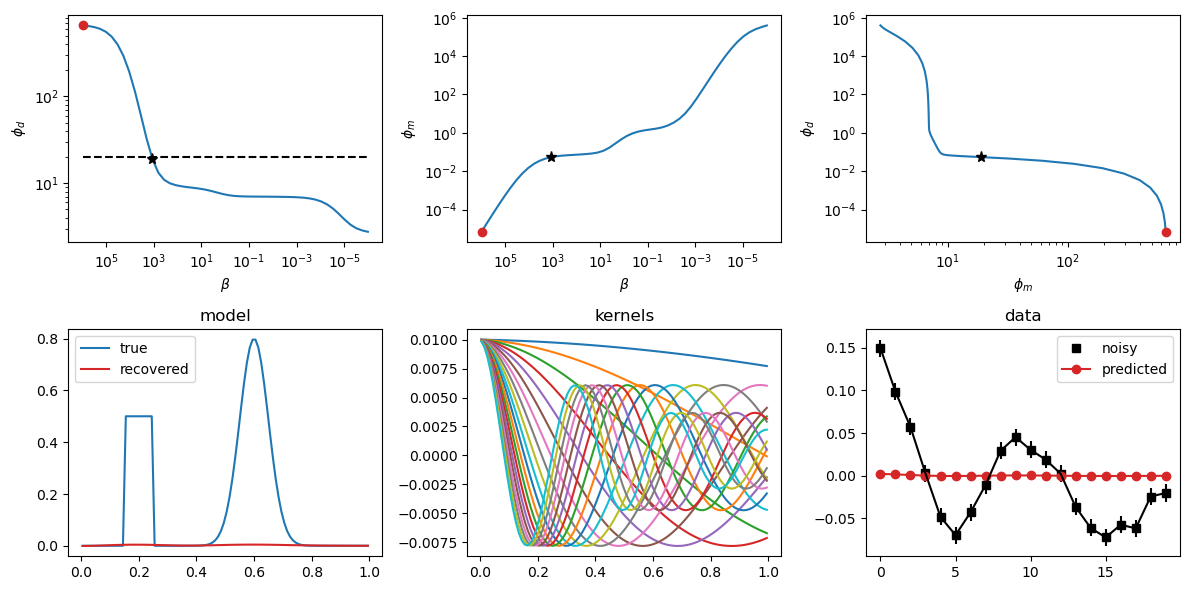
\includegraphics[width=0.7\textwidth]{Tikhonov-curves-example.png}
        \end{center}
    \caption{
        Example plot showing Tikhonov curves and the recovered model, kernels and data.
    }
    \label{fig:Tikhonov-curves-example}
    \end{figure}
}

\part{
    Create a vector that contains 50 values of $\beta$ that are logarithmically spaced between $\beta=10^6$ and $\beta=10^{-6}$. Set $\alpha_s = 1$, $\alpha_x = 0$ and plot the Tikhonov curves. On the plots for the Tikhonov curves, plot a line where the target misfit is and use a star to indicate the $\beta$ that corresponds to the largest $\beta$ where we have reached the target misfit (e.g. the largest beta where $\phi_d \leq N$, similar to Figure \ref{fig:Tikhonov-curves-example}). Choose 3 locations along the curves to show: one that is underfit, one that is overfit and one that acceptably fits the data. Choose examples that aren't at the total extremes. Describe which is which.
}

\part{
    Repeat the exercise from Q3a, but now set $\alpha_s = 0$, $alpha_x = 1$. Again, choose 3 examples, one that underfits the data, one that overfits the data and one that acceptably fits the data. Try to choose these models such that the $\phi_d$ values are similar to those for the choices you made in part a. Describe what is similar / different between the two scenarios.
}

\part{
    Time to play! Increase or decrease the noise, and discuss how this changes the Tikhonov curves, where the target misfit is and the nature of the model. Or what happens if you change the kernels and make them more / less oscillitory? or what if the decay more / less rapidly. Pick something to explore and generate a few plots to illustrate what you learned. I am expecting something no more that 2-3 plots that illustrate whatever you choose to explore.
}

\question{Finally, we will set up and solve the inverse problem using Singular Value Decomposition (SVD).}

\part{
    Perform the SVD decomposition of the system matrix $\mathbf{G} = \mathbf{U\Lambda V}^\top$. Generate a plot with 2 panels, show the singular values (on a log scale) and plot the first few singular vectors (use different colors to highlight which vectors correspond to each singular value)
}

\part{
    As we discussed in class, the model can be constructed from the singular values and vectors according to
    \begin{equation}
        \mathbf{m}_c = \sum_{i=1}^p \left(\frac{\mathbf{u_i}^\top \mathbf{d}^{obs}}{\lambda_i} \mathbf{v_i}\right)
    \end{equation}
    Create a function that returns $\mathbf{m}_c$ given the matrix $\mathbf{G}$ and a choice of the number of singular vectors, $p$. Generate a plot that shows: (a) the singular values, (b) the data misfit as a function of the number of singular vectors used to construct the solution (similar to the top left plot in Figure \ref{fig:Tikhonov-curves-example}, but replacing $\beta$ on the x axis with $p$, (c) the true and predicted models, and (d) predicted and observed data.
}

\part{
    Using the code you wrote for Q4b, show 3 different choices of the number of singular values: one that underfits the data, one that overfits the data, and one that acceptably fits the data. Specify which is which.
}

\part{
    Time to play! Change the kernels: what happens if you change the kernels and make them more / less oscillitory? or what if the decay more / less rapidly. Pick something to explore and generate a few plots to illustrate what you learned. I am expecting something no more that 2-3 plots that illustrate whatever you choose to explore.
}
\end{document}
% ========================================================= %



